%% LyX 1.1 created this file.  For more info, see http://www.lyx.org/.
%% Do not edit unless you really know what you are doing.
\documentclass[english]{book}
\usepackage[T1]{fontenc}
\usepackage[latin1]{inputenc}
\usepackage{babel}
\setcounter{secnumdepth}{3}
\usepackage{graphics}

\makeatletter

%%%%%%%%%%%%%%%%%%%%%%%%%%%%%% LyX specific LaTeX commands.
\providecommand{\LyX}{L\kern-.1667em\lower.25em\hbox{Y}\kern-.125emX\@}

\makeatother
\begin{document}

\title{OpenSG Starter guide}

\maketitle
\tableofcontents{}


\chapter{Introduction}


\section{What is OpenSG}

OpenSG is a real-time rendering system based on a scenegraph metaphor.
It works along the lines of OpenInventor, Performer or Java3D, although
it is probably closest to Performer. It supports parallel processing,
albeit in a more general way, and will drive multiple displays for
multi-screen stereo projection systems. The goal is to have something
that handles multi-threaded data structures as simply as possible
without compromising performance too much. It should also support
heterogeneous multi-pipe applications, i.e. multiple different graphics
cards running one application. Many things are quite easy to do with
a little program, but are sometimes hard to fit into an existing system.
Thus accessibility is an important goal, and we're striving to make
OpenSG very extend-able.

It works on different Unix systems and Windows. 

It's primary use (i.e. what we are doing with it) is for VR applications,
mainly in the automotive context. But it can be used for any kind
of application needing fast and general 3D graphics. 


\section{What is OpenSG not}

OpenSG is not a complete VR system. Things like device access and
interaction are left out on purpose, there are other systems for that.


\section{Where do get it}

www.OpenSG.org blabla


\section{How to compile and install}

INSTALL/README blabla


\section{How do use it}


\subsection{Own projects}

Makefile blabla


\subsection{Extending OpenSG}

Makefile blabla

test files


\chapter{Working with OpenSG}

only overview, look at the doxygen files for detailed description
blabla


\section{Base types}

Platform Independence blabla


\subsection{Log}


\subsection{Math (vector,point,matrix,quaternion)}


\subsection{Image}


\subsection{Threads}


\section{Fields and FieldContainer}

container for everything that is thread-save


\subsection{Createing new Field Container classes}

fcdEdit (see image \ref{fcdEditFig}
\begin{figure}
{\centering \resizebox*{0.9\columnwidth}{!}{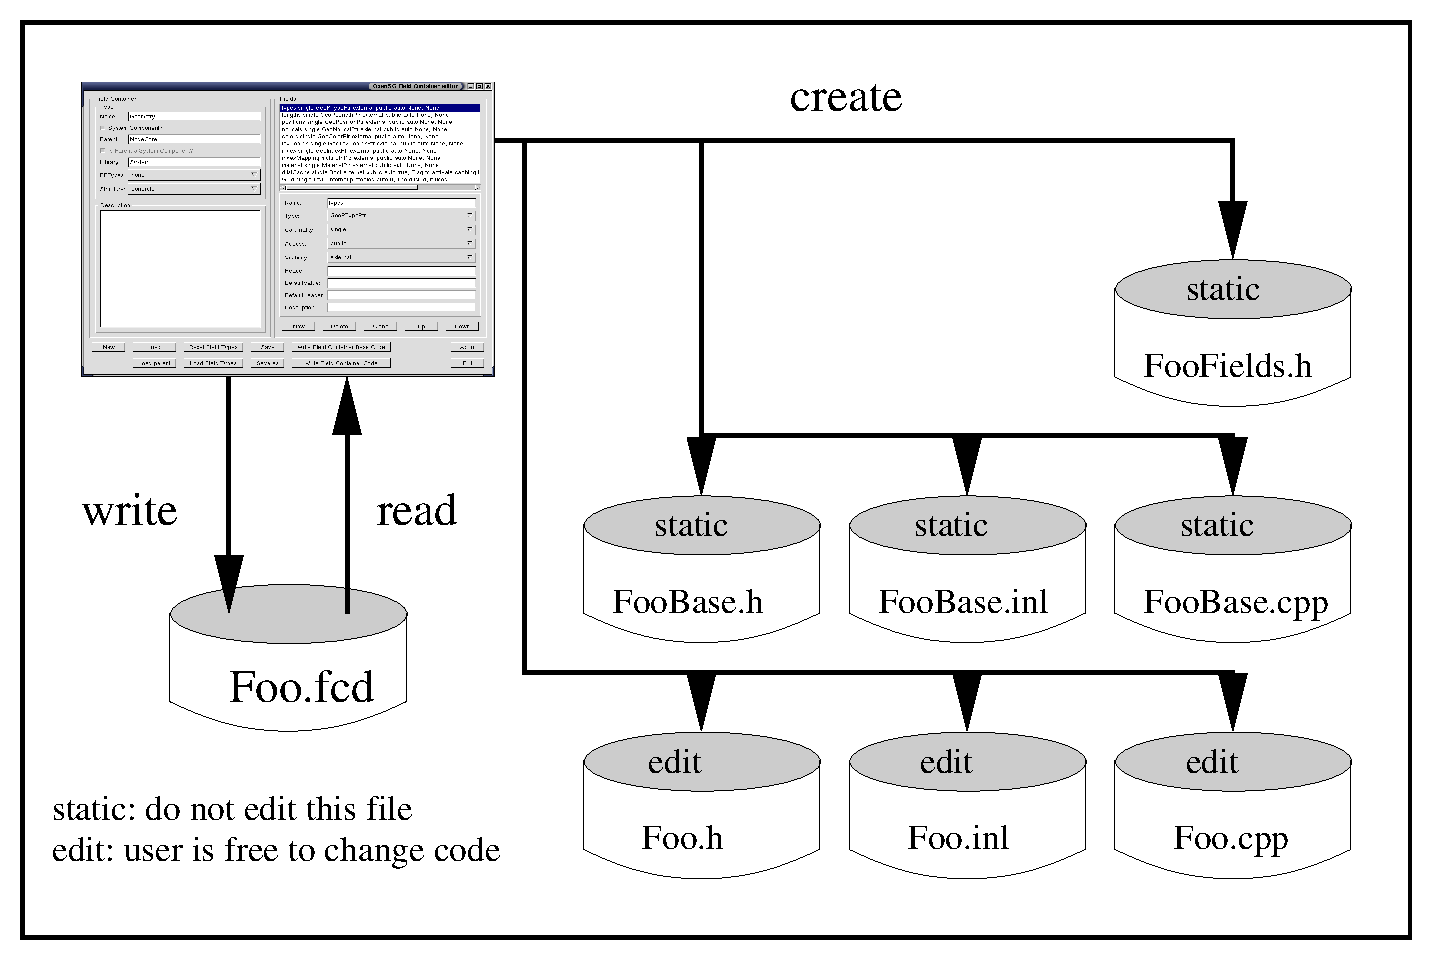
\includegraphics{fcd.eps}} \par}


\caption{\label{fcdEditFig}FcdEdit blabla}
\end{figure}
 ) stuff


\subsection{Creating a FieldContainer instance}

factory,prototype blabla


\subsection{Changing field values}

changelist blabla


\subsection{FieldContainer attachments}

attachment blabla


\section{Nodes and NodeCores}

single (see image \ref{singleParentFig}
\begin{figure}
{\centering \resizebox*{0.8\columnwidth}{!}{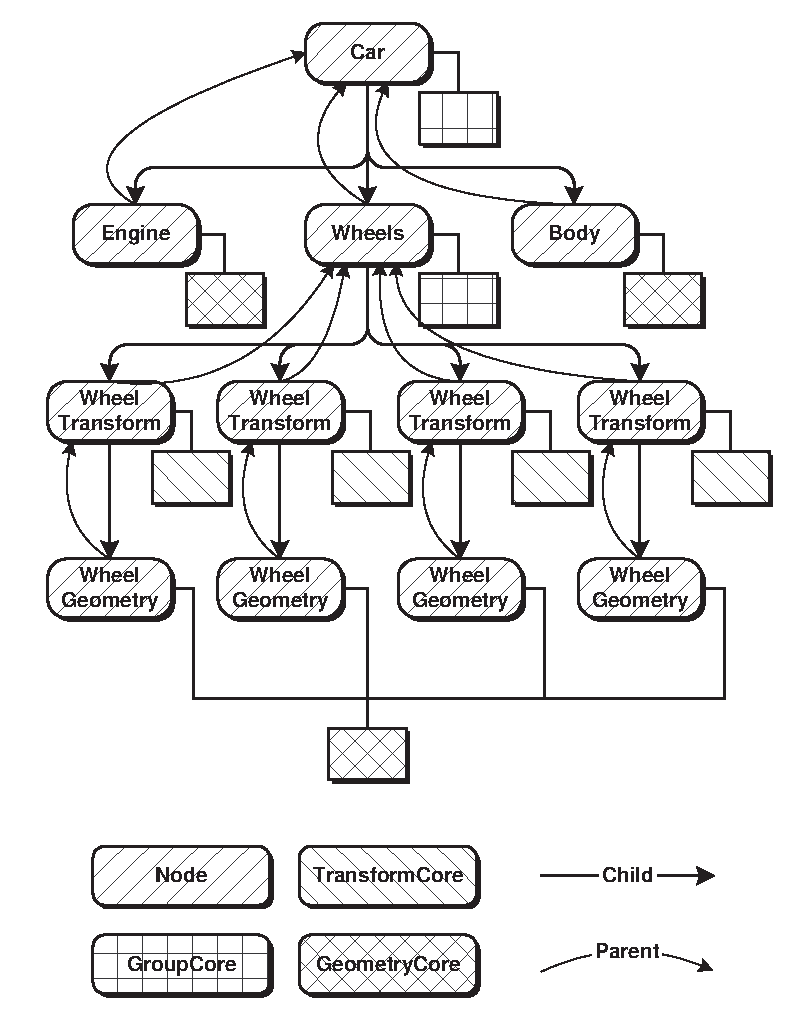
\includegraphics{node_core_share.eps}} \par}


\caption{\label{singleParentFig}Single Parent Scene}
\end{figure}
) /multi-parent (see image \ref{multiParentFig}
\begin{figure}
{\centering \resizebox*{0.8\columnwidth}{!}{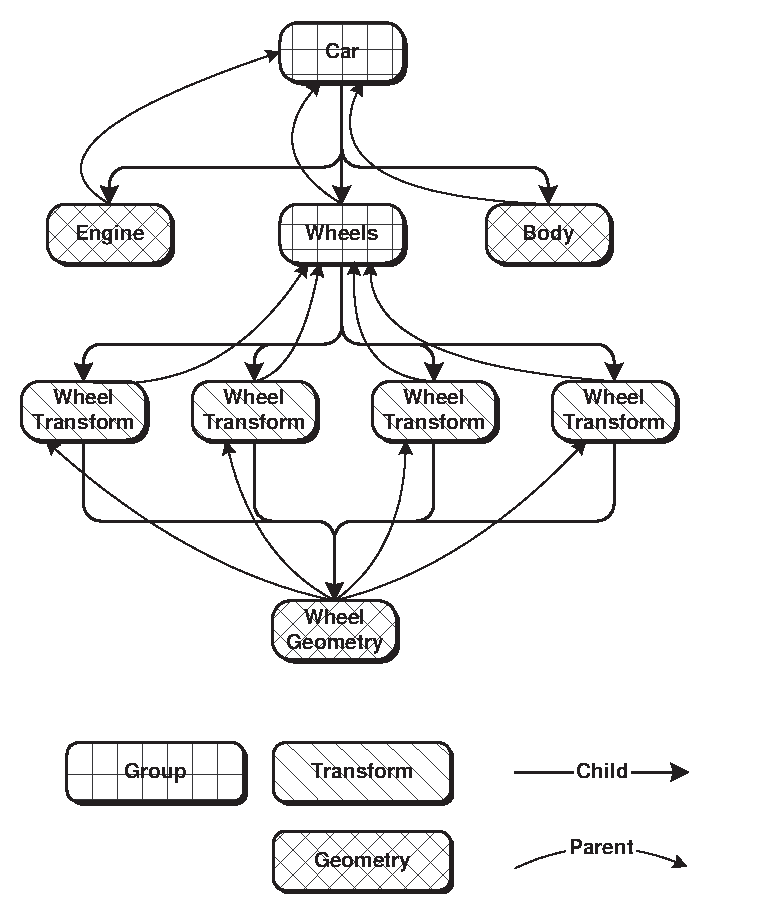
\includegraphics{tree_multiparent.eps}} \par}


\caption{\label{multiParentFig}Multi Parent Scene}
\end{figure}
) stuff


\subsection{Node }

volume stuff, toWord matrix


\subsection{NodeCore }


\subsubsection{Special Node Cores}

\begin{description}
\item [Material]chunk stuff
\item [Geometry]property stuff
\end{description}

\section{Action and Traversals}


\subsection{Usage}


\subsection{Write our own action handler}


\subsubsection{Camera and Window}


\section{Loader}


\subsection{Usage}


\subsubsection{Scene}


\subsubsection{Image}


\subsection{Write our own}


\subsubsection{Scene}


\subsubsection{Image}
\end{document}
